% to cite stuff use \cite{cite_key}

% Heirarchy:
%\part{part}	-1
%\chapter{chapter}	0
%\section{section}	1
%\subsection{subsection}	2
%\subsubsection{subsubsection}	3
%\paragraph{paragraph}	4
%\subparagraph{subparagraph}	5

\documentclass{article}
\usepackage{times}
\usepackage{cite}
\usepackage[autostyle]{csquotes}
\usepackage{marginnote}

% to avoid having to escape all underscores to avoid "missing $ inserted" error.
\usepackage{url}

%\textwidth = 490pt

\usepackage{graphicx}
\DeclareGraphicsExtensions{.pdf,.png,.jpg}
\graphicspath{ {./figures/} }

\setlength{\parskip}{0.6em}

\begin{document}

\title{Bringing Knowledge Through AI and SMS}
\author{Sam Heather\\
  Department of Computer Science,\\
  The University of York,\\
  \texttt{sam@heather.sh}}
\date{\today}
\maketitle

\newpage

\begin{abstract}

\marginnote{It is early days so it is normal that many things are missing from the abstract. You should keep in mind that it should include later on few sentences on method/experiment, result and conclusion.}

In remote Africa, there are millions of disadvantaged and uneducated individuals, who, in the vast-majority, do not have access to the internet and the access to knowledge that this brings.  Outside of their immediate friends and family, individuals can not get access to the information they need on anything from their own body to social problems.

In many parts of the world, the number of people without access to the internet, but access to a mobile phone, is significant.  This project aims to research and develop a system capable of bringing knowledge through a question and answer based interactive system, in the language natively spoken by the user, through the use of a simple Artificial Intelligence and an SMS interface.  The system will be expandable, such that it can be adjusted to handle questions on any knowledge area.

This project raises ethical issues relating to the responsibility of providing accurate information when in a position of trust, the ethics of machine translation and maintaining user privacy.
\end{abstract}

\newpage
\tableofcontents
\newpage
\listoffigures
\newpage
\listoftables
\newpage

\section*{Statement of Ethics}
% TODO write this
{\bf Pretty much the most important part - write this!}

\newpage
\section{Useful thoughts from Lilian}
Take a quick look at list of other students previous projects to get an idea of how intro/lit review is structured etc.

Remove page number on title page.



Remember to take notes on when I come across problems, for my conclusion.

\section{Introduction}

\subsection{Background of this project}

The inspiration for this project originates from a project the author undertook in September 2014 whilst attending a week long 'hackathon' (Yacht Hack, http://toughhackers.com/yacht-hack-2014/), with Julie Markham and Nicholas Hopper, called Shy.  On this project, the author co-created a project to prototype a mobile application that would facilitate the immediate answering of questions that fall within certain categories.

One of the initial aims of Shy was to further the transition from e-learning (learning conducted online, usually with the help of a computer) to m-learning (learning using tools available on a mobile device).  M-learning is an especially important topic at the moment, due to the high, and increasing, availability of mobile devices worldwide.

A semi-functional prototype was completed for iOS (shown in Figure~\ref{fig:shy-ios-screenshots}), although question recommendations were evaluated without knowledge of previous material the user had viewed, and as such there was no knowledge of their interests to support explicitly targeted answers for a question they might search for.

Up until this point, the service was restricted to working on iOS smart devices only, with poor quality question/answer matching.

{\bf should add at least one more significant paragraph here, not sure what to write about though}

\begin{figure}[htb] 
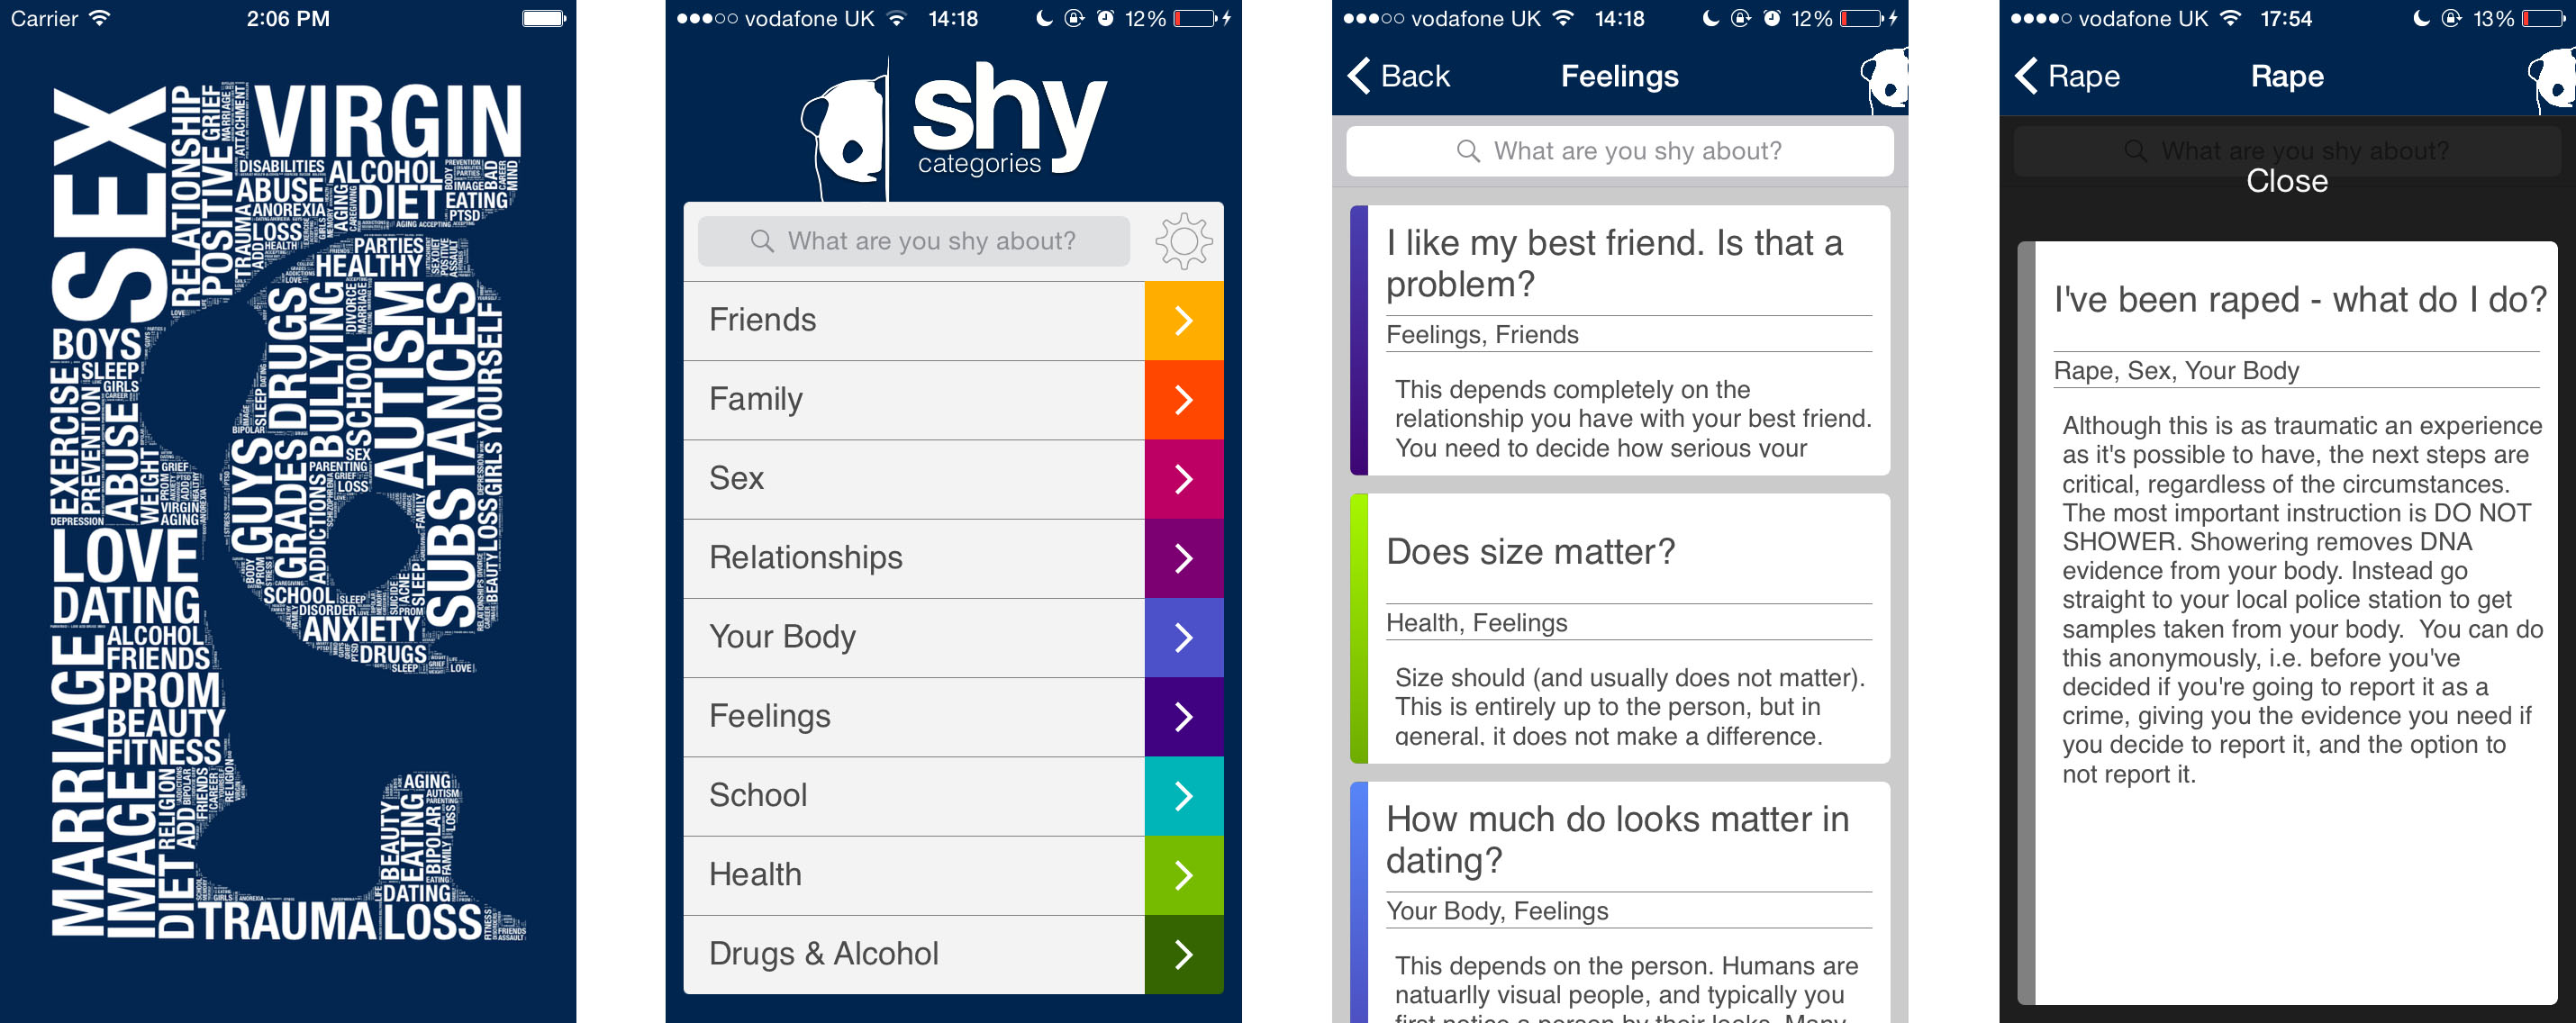
\includegraphics[width=\linewidth]{shy-screenshots}
\caption{Screenshots of Shy iOS App}
\label{fig:shy-ios-screenshots}
\end{figure}

\subsection{Motivation for this project}
Access to knowledge is, in the opinion of the author, a critical part of modern life.  It's also a Human Right, under Article 27 of the Universal Declaration of Human Rights~\cite{community1948universal}.  Indeed, we use tools to access knowledge hundreds of times each day, often unaware that we are doing so.  Despite this, hundreds of millions of individuals live without this facility.  This project aims to investigate and create a technology to give more people access to knowledge, and thus their human rights.

The project also involves the use of a number of systems to work, including machine translation, an SMS input/output system and a custom system to build a profile on a user, to facilitate high-quality question-answer matching.  These, along with complex ethics and privacy issues create an interesting project that draws together many technologies and discussions in a way that can be used as a basis for other projects in the future.

\subsection{Aims of this project}

The first goal of this project is to assess and address the ethical issues that arise from the software that this project aims to create.  These include the responsibility the software has, stemming from it's position of trust, to provide accurate information and protecting the privacy of users by using only necessary information, among others.  The author will do this by researching ethical issues relating to the technologies that the project will use, for example machine translation.  This will then be used to feed the design process of the software and to specify the expected use-case of it.  Finally, the resulting software will be evaluated through experimentation, with volunteers been asked to ask a set of questions within a topic area, in a non-English language, and evaluate the relevance of answers returned.

\subsection{Structure of this report}
This report starts with a review of pre-existing literature on this topic, in chapter~\ref{sec:literatureReview}, where the author looks at existing software, tools and services of a similar type to those that will be either used in this project or that which this project hopes to create to research the problems that they stumbled across.  Comparisons between different software development life-cycles are also discussed.

Chapter~\ref{sec:method} describes the method that will be taken to develop the software and service.  This covers the software development life-cycle that will be followed, and sets out a plan for when development will take place.  Requirements will also be identified, described and categorised  as either functional or non-functional.  A method of evaluating the success of the software will also be discussed and chosen.

The design of the software, driven from information collected from the requirements, will be set out in Chapter~\ref{sec:design}.  The individual components that make up the technology will be described and discussed\marginnote{described and discussed, or just described?}, followed by a description of how these modules will interface with each other to build a complete system.  Finally, this section will include a description of the platform, language and other tools that will be used.

Chapter~\ref{sec:implementation} contains details about the implementation of the software.  This includes information on the tools that were used to create components such as the SMS interface and question/answer matching system.

Results from the evaluation of the system will be presented in Chapter~\ref{sec:results}.  A discussion of these results and their implication on this project is then presented to the reader in Chapter~\ref{sec:discussion}.

Chapter~\ref{sec:evaluation} contains an evaluation of the software produced and the process taken to complete it.  Comparisons will be made to the success criteria, set out for the project in section <insert number here>.

The authors thoughts on potential future work, building on the work produced in this project, are then displayed in chapter~\ref{sec:extending}.  

Finally, the main achievements of this project and then the report is concluded in chapter~\ref{sec:conclusion} with final thoughts.


% Lilian: This section should be expended, especially mentioning the consequences of such assumptions. Why do you make those assumption (e.g. time constraint, little or no consequences, ...). What limitation this may cause to your findings.  Shows a mastery of the field.
\subsection{Assumptions Within This Project}
This project will make the assumption that users of this service have basic literacy skills in a language supported by the project.  Although this is not true for the whole of Africa, expanding the remit of this project to include a 'graphical' user interface that works over SMS is a challenge larger than would fit in an undergraduate dissertation.

\newpage

\section{Literature Review}
\label{sec:literatureReview}

{\bf The point of this is to show that I 'own' the material and subject (competence).  Show different points of view, choose a side, express a view on which I prefer and if I agree, critique.  Have objective goals.}

% expand introduction to explain why sms, then look at related work in next section.  compare to smart phones loosely.
A significant amount of work has previously been undertaken in the area of making knowledge quickly accessible to us in the form of questions and answers.  To take one example, consider the situation of suspecting that a relative was suffering from a disease, for example, Cholera.  The initial step would be to search for information before seeking medical assistance.  In the connected world, this is easy - a simple Google search returns the answers, as shown in Figure\ref{fig:cholera}.

\begin{figure}[htb] 
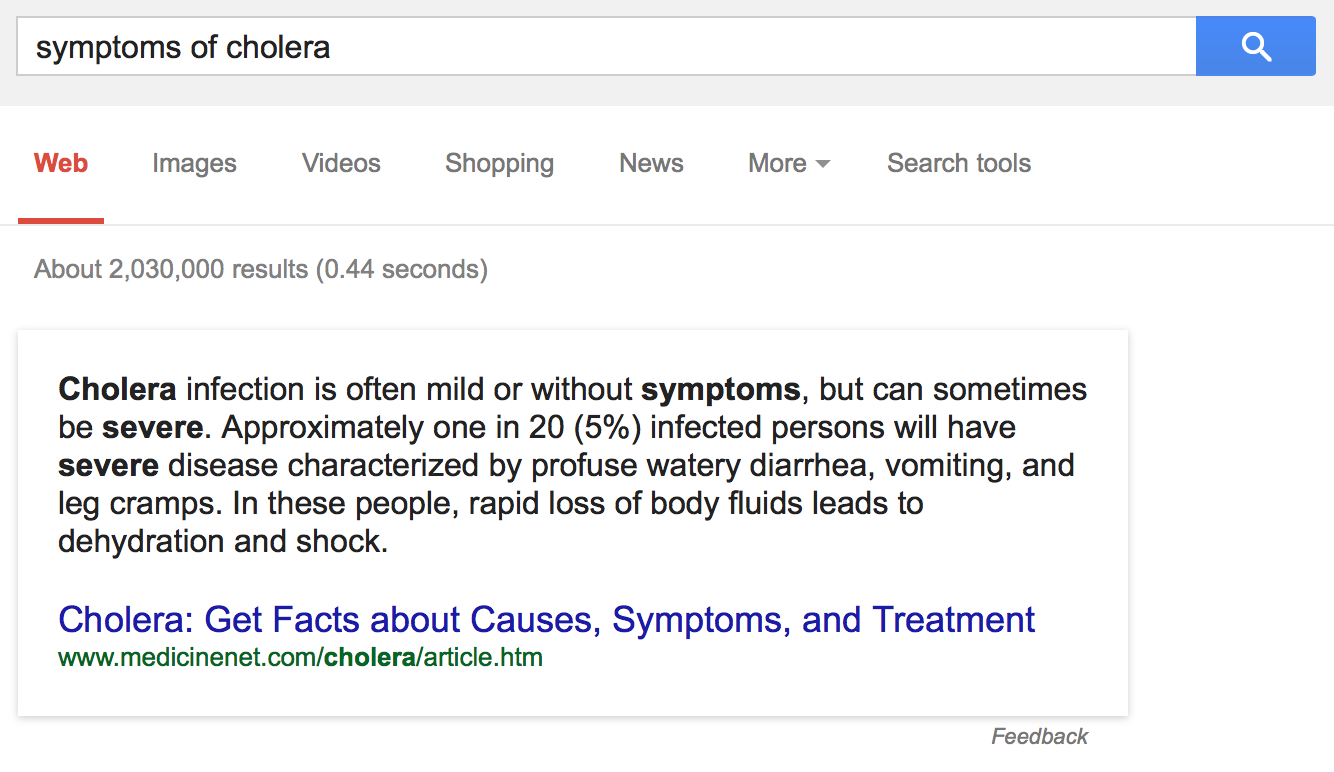
\includegraphics[width=\linewidth]{googleCholera}
\caption{Google Now information box}
\label{fig:cholera}
\end{figure}

% Lilian: You should give a caption to all figures and tables. use \label{fig:WebQuery} after \caption{Web query result for "Symptoms...}  for example. In this instance you should mentioned the date you made the query and which search engine you have used.

This is easy to do in the developed world, where up to 75\% of the population are connected to the internet~\cite{ITU_Cell_Usage_2013} (with the population of elderly people been largely responsible for the remaining 25\%~\cite{Gov_Internet_Usage_UK_2014}).  This contrasts strongly with the situation in the African continent, where, in 2013, internet usage had only reached 16\%~\cite{ITU_Cell_Usage_2013}, a figure largely inflated by South Africa, where 5\% of the African population generate 2/3 of internet traffic from the African Continent~\cite{ITU_Cell_Usage_2013}.

% But there are other communication methods which are proven to work
\subsection{Previous work using SMS}
Although the above suggests that the African continent is majoritively disconnected, this is not the case.  Because of restrictions in the electricity available, the ways in which a mobile phone can be used in Africa have far surpassed those in the developed world~\cite{Fox:2011:Online}, in-part due to the low power consumption of a mobile phone.  Interesting such examples include automated services which SMS HIV/AIDS sufferers, reminding them of medication to take, and providing access to current market information for agriculture and farming, saving farmers from making daily trips (often many kilometres) or relying on out-of-date information from a weekly radio broadcast~\cite{Aker_Mobile_Phones_2010}.

Interactive systems have also been developed to operate over SMS.  One successful example includes mobile money platforms.  These allow for users, from any background, to pay and be paid for goods, and to transfer money across long distances, at negligible cost~\cite{Aker_Mobile_Phones_2010}.  One of the most highly adopted services is M-Pesa - which, in Kenya alone, was responsible for \textsterling5.7 Billion in transfers in 2012 \footnote{Data from Safaricom, M-Pesa operator in Kenya - actual value 817,085,000,000 Kenyan Shillings, converted to GBP on 1st November 2014 at rate of approximately 0.007.}.  M-Pesa gives users a balance linked to a national ID number, from which they can pay for goods by sending an SMS with a cashier (recipient) number or pay outstanding bills in a similar way.  Non-subscribers can also use the system, by depositing money with a M-Pesa cashier in exchange for an access code, which can be sent via SMS to a contact, who can subsequently redeem it with their local cashier~\cite{Aker_Mobile_Phones_2010}.

This difference in standard use of cell phones is demonstrated in the International Telecommunications Unions's 2013 report~\cite{ITU_Cell_Usage_2013}, which shows that in Europe, for 790 million mobile subscriptions, 53\% of subscribers have mobile internet access (422 million), compared to 17\% in Africa (93 million have mobile broadband, out of 545 mobile subscribers).  This is due to the prohibitively high cost of accessing data services, regardless of the hardware that the user has.  In 2012 in Europe, 500 MB of data per month for 12 months cost 1.2\% of the average Gross National Income Per Capita (GNI pc).  In Africa, the average price was 30x this, at 36.2\% of an individuals GNI pc~\cite{ITU_Information_Society_2013}.

% No research has been undertaken investigating whether bringing knowledge through this method is viable option.

\subsection{Ethical Issues}
This project raises a swathe of ethical issues related to translation accuracy, providing information to people in an ethical way and maintaining user privacy.

\subsubsection{Ethics of Providing Information}
One significant issue for this project stems from providing information that may affect an individual or lead them to take a harmful action.  {\bf In a similar way to that which a teacher has a responsibility to teach accurate information to a pupil, due to their position of trust, any service relied upon by a user must equally provide accurate information.  The result of not doing this could be providing inaccurate information that leads to a user carrying out an action that causes harm}.% TODO Reword last two sentences.  This is something imporant and obvious - perhaps simple analogy is not necessary.  Perhaps give a generalised example.

% Lilian: You may want to look toward news paper (online/printed) to look at current/past issues that led to a law suit/inquiry and subsequent verdict/laws that may have been changed.

% Lilian: You should provide both point of view so do use this material, then you will have to critic both point of views. 
{\bf this needs to be waaaayyyyy expanded, but I struggled to find information that was useful.  There's lots on remote education, and on basic ethics of teaching, but I struggled to find anything specifically relating to ethics of ensuring information you provide is correct (actually I found some material that pointed the other way)}.

\subsubsection{Ethics of Translation}
A significant part of this project is represented by the support of multiple languages.  It is clear that translation on demand, at scale, needs to be automated by some kind of machine or algorithmic translation.

This project involves two blocks of translation.  These are:
\begin{itemize}
  \item The translation of the user's input into the language of the system (English)
  \item The translation of the answer to a users question from the system language to their local language.
\end{itemize}
The second of these raises some issues.  To understand these, it is necessary to first understand the two categories of machine translation.

Rule-based machine translation effectively treats human language in a similar style to programming languages.  Formal grammars and lexicons are used to represent words that exist in either the source or target language, structures representing the translation of individual words or groups of words.  Map structures map individual or groups of words to their translated counterparts, sometimes with multiple results (a 1-many map), from which rules decide which is selected.  Maps and rule sets are created by trained computational linguists~\cite{kenny2011ethics}.

More commonly, Statistical Machine Translation (SMT) is used (for example, this is used by Google and Microsoft Bing Translate)~\cite{kenny2011ethics, Google_Translate_Research}.  Statistical machine translation learns maps between strings of words of potentially non-equal lengths from pre-existing original texts and their trusted human translations.  The accuracy and breadth of language support for translation increases as more source material is analysed by the system, as potentially erroneous or low quality translations can be identified and marked.  SMT is also dependent on the quality of the human translation on the input material~\cite{kenny2011ethics}.

The aforementioned issue that is present in statistical machine learning systems comes from the knowledge we assume an individual has and derives from a word.  In human translation, this is solved by the translators knowledge of the difference in material culture, allowing them to append necessary information to the resulting translation that the recipient might find useful.  In statistical machine learning, cultural awareness of material knowledge is a separate problem on it's own, on this scale.  {\bf formal reference to this, probably again from Kenny, but should be able to find better}.  To take one example, from Melby (2006),

\blockquote{"when translating a French menu, a human translator might stop to think that an English speaker in France would appreciate being told that a steak tartare is served entirely raw, even if this information is not contained in the original text (because French people might be assumed to know this already). Such a translator would be aware of differences in material culture, and would be able to empathise with the English speaker who might choose to avoid the dish, given more information"~\cite{melby2006can, kenny2011ethics}}
\marginnote{Lilian: quote taken from~\cite{kenny2011ethics}, but quote is interpreted from~\cite{melby2006can} - so I think referencing both is correct, but for this reason rather than last reason we discussed?}

This issue is a result of the translation engine not been capable of taking as input, and using, a complete representation of the expected cultural differences between those who speak the input language and those who speak the output language~\cite{melby2006can}.

{\bf below should really be expanded and be in the discussion.  Explain the decision to keep translated answers in the database, which are pre-approved, to ensure no cultural misunderstandings.}

Because the potential use of this system, regardless of whether this is within this project or by a third-party using the results of this project upon completion, could include distributing information that may be used by an individual making an important decision, cultural confusion such as this could have potentially catastrophic effects.

\subsubsection{User Privacy and Data Protection}
This project uses a simple Artificial Intelligence (AI) to keep a record of information that has already been returned to a user, to attempt to save sending repetitive information (saving the cost of additional SMS).  This raises another ethical issue though - a privacy issue.  The material that a user has researched is likely to be sensitive - such is the nature of health related questions.  This means that the information on a user has to be kept securely, in a way that an individual user can not be identified.

One way of doing this is using a technology called hashing.  Ideal hashing is the technique of taking data as an input and generating an output value (called a 'hash') that is unique to an input.  Hash functions are ideally one way functions, where given input data X, the output hash will always be Y, whenever and however the hashing algorithm is executed.  This allows a users identify (phone number) to be obscured (hashed), in such a way that the mobile number can not be recovered from the database.  When a question is received, the phone number (represented by variable X in the above example) can be hashed and the data for this number looked up from the database, without the database application ever been aware of the phone number of the user.  In the example in Figure~\ref{fig:hashPhoneNumber}, a phone number (X) is used as input to an imaginary hashing function and the output hash (Y) is shown on the right hand side.  As just described, this number can then be used as the key for the user information database, shown in Table~\ref{table:hashDatabase} to retrieve the information needed for the AI.

{\bf reference the above from security engineering ross anderson, chapter 10 and 21?}

\begin{figure}[htb]
    \centering
    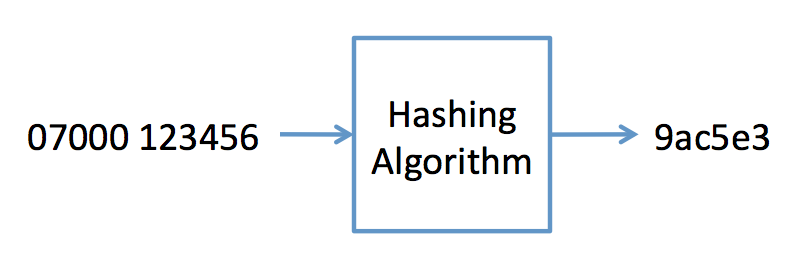
\includegraphics[width=200pt]{hashPhoneNumber}
    \caption{Hashing a phone number using an imaginary hashing algorithm}
    \label{fig:hashPhoneNumber}
\end{figure}

\begin{table}
\begin{center}
    \begin{tabular}{| l | l |}
    \hline
    userId & userData \\ \hline
    8f64B2 & \{‘previousQuestions’:[13,301,170,577]\} \\ \hline
    9ac5e3 & \{‘previousQuestions’:[441,56]\} \\ \hline
    f9dd7e & \{‘previousQuestions’:[301,623,89,280,364,621,209]\} \\
    \hline
    \end{tabular}
    \caption{Example of software database: hashed phone numbers paired with a list of previous returned answer ID's. }
    \label{table:hashDatabase}
\end{center}
\end{table}

In practise it is possible for the output of a hashing algorithm not to be unique to a particular input.  This is because the range of possible input values is much smaller than the range of output hashes, and because all valid inputs must map to an output, there is repetition in outputs~\cite{mitCryptographyMd5}.  This property of hashing algorithms can be a security risk for some use-cases, where hashes are used to verify that data has not changed since been hashed.  In this case, a third-party may be attempting to generate alternative, malicious data with the same hash as some pre-existing data, to swap them unnoticed~\cite{securityEngineeringHashingAnderson}.  In the use-case of this project however, hashes are only been used to anonymise phone numbers to some unidentifiable string of characters and numbers, meaning that the above-described collision risk is not a security risk.

Two properties that this project does need from it's hashing algorithm are collision resistance and irreversibility.  Collision resistance the property of a hashing algorithm that determines the probability of the same output hash for two distinct random inputs~\cite{mitCryptographyMd5}.  A high collision resistance is necessary to ensure that two users of the system with distinct phone numbers don't get mapped to the same row in the database, resulting in poor quality question/answer matching.

Irreversibility is a necessary property of the hashing algorithm chosen for this project.  This ensures that the key used in the database can not be used to retrieve the phone number of the user, thus protecting their identity.  Commonly used hashing algorithm families, such as the MD family (e.g. MD5) and SHA family are all designed to be one-way~\cite{schneierCryptanalysisMD5SHA}\footnote{Bruce Schneier is a fellow at Harvard's Berkman center for internet and society.  He has been posting regularly for his newsletter and then blog since 1998 (over 16 years) and has published material related to this field throughout this time.  He has been involved in the creation of other cryptographic algorithms, such as the Skein hashing algorithm, blowfish block cipher, so may have a vested interest in dis-crediting other algorithms such as MD5 and SHA.  However, the essay cited above is written as a result of the Crypto 2004 Conference in California, Schneier has a world-renowned reputation for cryptography and computer security and the algorithm that he suggests should be used at the end is not one that he has involvement in.  For these reasons, I believe this source is reliable.}.  

Although hashing algorithms are computationally one-way, they can suffer from another type of vulnerability affecting the security of the original input data.  When hashes are used for short strings of information (passwords, for example), a simple way to try and retrieve the original data is to compute a dictionary of the hashes of lots of common passwords, from which matches can be found.  This idea has been extended to produce Precomputed Hash Chains and subsequently Rainbow Tables.  These are highly efficient data structures that consist of chains of processed input messages and their hashes (with a reduce function to reach the next item in the chain), allowing original input data to be looked-up from it's hash.  Both Precomputed Hash Chains and Rainbow Tables tend to be Terabyte's in size, and as such they only exist in a significant form for the most common hash functions (including MD5 and SHA) ~\cite{Teat:2011:SCH:2016039.2016072}.  Within this project, this raises privacy implications, as hashes within the database would be 'convertible' to phone numbers.  

{\bf perhaps the below should move to method and requirements - TODO needs to be cleaned up as well.}

In modern password authentication, a tool called bcrypt is used, which 'salts' passwords (additional unique data is added to each password before hashing), nullifying the use of Precomputed Hash Chains and subsequently Rainbow Tables.  However, this would prevent efficient lookup of phone numbers in the communications part of the application (where answers and sent back to the user).  As such, the best way of protecting a users phone number in the event of a database hack is to use a combination of a largely uncommon hashing algorithm, on the basis of it is unlikely anybody will have wasted vast computation power for a table that's useful in such a small number of situations, a hashing algorithm with a large output size, again because it makes a table more infeasible (because of size constraints) and a further change to the output hash, specific to this application.  This way, a hacker would need to know this change (from the source code) as well as the password database, to be able to make use of a hashing table.  The above is commonly implemented by hashing the result of one hash with another hashing algorithm.

\subsection{Software Design Life Cycles}
{\bf Describe and compare some software design life-cycles} %TODO Describe and compare software design lifecycles
There are many software development life cycles that a developer or company has available for them to choose from.  Four common ones include the Waterfall Model, Iterative Model, Spiral Model and the Agile Development Model.\marginnote{Do I need to reference that these are common?}  In order to choose which life cycle suits this project best, research into all four has been carried out.

\marginnote{Should this be in this section, or moved to the "Method and Requirements" section?}

\subsubsection{The Waterfall Model}
The waterfall model consists of 5 phases of work, where each leads directly into the next.  It is a plan driven development model, which means that all process activities such as the implementation of the project must be planned and scheduled before work on them begins ~\cite{sommervilleSoftwareEngineering}.  The five layers in the model are:
\begin{enumerate}
  \item Requirements.  In this stage, both user and system requirements for the project are determined after examining the business goals for the project.  These form the system specification.
  \item Design.  In this stage, a plan for the software development is created.  The overall architecture for the software is created, the external libraries to be used are chosen and the interaction between different modules is modelled.
  \item Implementation.  In this stage, the software is implemented to match the design and architecture set out in the Design phase.  Unit tests are written to ensure that each module matches its specification.
  \item Testing.  In this section the system is tested as a whole to test for any bugs that might not be picked up when testing individual modules in isolation.  The software is then delivered.
  \item Maintenance.  Finally, the software is deployed and maintained.  This includes making changes to the requirements and subsequently the software (implementation) as the business goals change.  ~\cite{sommervilleSoftwareEngineering}
\end{enumerate}

Because the waterfall model is so fixed and progressive (once development has moved from one stage to another, it can not go back)
%TODO add main advantage
%TODO add main disadvantage

\subsubsection{The Iterative Model}
Iterative development is the practise of splitting the overall development of a project into multiple independent and distinct blocks.  A block contains a sequence of tasks (essentially a mini life cycle) such that each iteration can really be thought of as it's own project.  Each iteration tends to focus on a specific set of features, such that when the iteration is complete the overall project is stable and the modules developed to-date can be tested as a whole system ~\cite{differenceBetweenLifeCycleModels}.

There are a multiple variations of the iterative development method, including Timeboxed Iterative Development (where all iterations have a fixed, inflexible length) and Client-driven Iterative Development (where each iteration contains the features that the client considers have the highest business value) ~\cite{larman2004agile}.

A common variation is based on the waterfall model, and is shown in Figure \ref{fig:iterativeDevelopment}.  The first three tasks in the cycle represent the first four stages in the waterfall model (Requirements, Design, Implementation and Testing), at which point there is the option to either evaluate progress so far, and start another iteration, or to deploy the software and end development.  One significant difference between this and the waterfall model is that maintenance is not represented.

%TODO add main advantage
%TODO add main disadvantage

\begin{figure}[htb] 
\centering
    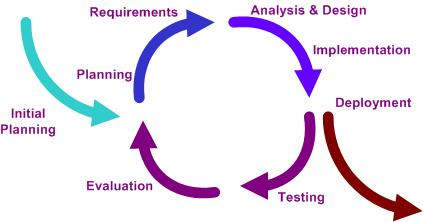
\includegraphics[width=0.8\linewidth]{iterativeDevelopment}
\caption{Iterative Development Method}
\label{fig:iterativeDevelopment}
\end{figure}

\subsubsection{Boehm's Spiral Model}
The Spiral Model was originally developed as a result of the adjustments that were regularly made to the waterfall model in large government projects ~\cite{spiralModelSoftwareDevelopment}.  The Spiral Model is a general model and can be used as a generator for other more specific models, given the parameters for a project such as it's risks ~\cite{boehm2000spiral}.  Models such as the waterfall model are specialisations of the spiral model ~\cite{boehm2000spiral}.

%TODO add main advantage
%TODO add main disadvantage

A detailed description on the spiral model can be found in Boehm's paper "A spiral model of software development and enhancement", where he published the complete concept ~\cite{spiralModelSoftwareDevelopment}.

\subsubsection{Agile Development}
Agile Development essentially represents a group of development techniques (such as 'Extreme Programming') targeted towards either the development of a small to medium sized product for sale or the development of a custom system within an organisation, where the customer has a high degree of involvement ~\cite{sommervilleSoftwareEngineering}.

Agile development is highly targeted towards teams, with components such as Pair Programming, Collective Ownership, regular meetings and employee health (avoiding overtime) playing an integral part in the model ~\cite{sommervilleSoftwareEngineering}.

\subsubsection{Development Life Cycle Summary}
Iterative development has been chosen as the model that this project will follow, based on the following factors:
\begin{enumerate}
  \item Boehm's Spiral Model and Agile Development are both targeted towards development teams.  A significant part of these models relates to team interaction, so they are not appropriate to this project.
  \item The Waterfall Model is rigid and inflexible.  It does not allow for the changes to the requirements and implementation that might be proposed after evaluating the quality of the first implementation.
  \item The Iterative development model can be implemented well by a single developer \marginnote{I need to add this as a 'pro' above}, and supports adjusting the requirements and implementation in each iteration of the cycle.
\end{enumerate}


\newpage
\section{Method and Requirements}
\label{sec:method}

\subsection{Chosen Software Development Lifecycle}
%TODO start writing this!

\subsection{Plan for Software Development}
%TODO start writing this!
Software development will follow the principles set forth in the iterative software development life cycle.  That is: Initial planning will take place 

\subsection{Requirements}

\subsubsection{Use Cases / User Goals}
%TODO Have I used use cases correctly here?
Two personas were created in Appendix Section \ref{sec:appendixPersonnas} to represent individuals who may have a need for the work resulting from this project.  From these personas, user goals are extracted.  These describe what a general user aims to achieve with this service.
\begin{enumerate}
  \item Nanjala wants to be able to read general information on any given topic.
  \item Ethan wants to be able to retrieve facts from direct questions.
  \item Both Nanjala and Ethan want to be able to achieve their goals entirely via SMS because of their circumstances.
  \item Ethan needs a simple and efficient user interface that allows him to retrieve facts quickly. 
  \item Ethan wants to be able to feedback into the system when he finds an answer particularly useful or unhelpful. 
  \item Nanjala wants to be able to show the service to her friends without explaining how to use it every time.
  \item Nanjala wants to get recommendations on content she might find interesting. \marginnote{Haven't decided yet if this is a feature I will implement - time based!}
\end{enumerate}

\subsubsection{User Requirements}
User goals are distilled into formal user requirements.  Each user requirement corresponds directly to the correspondingly numbered user goal.
\begin{enumerate}
  \item Users must be able to request general or descriptive information on a geographical entity.
  \item Users must be able to ask questions requesting a fact or statistic about an entity and get the answer or number they are looking for.
  \item Users must be able to interact with the system over SMS.
  \item Users must be able to make their queries and get responses quickly.
  \item Users must be able to feedback to the system when an answer is of noticeably low or high quality so the system can learn and improve.
  \item Users must be able to learn how to use the system themselves and this learning process should be quick.
  \item Users must be able to get recommendations on entities they might be interested in, based on previous query history.\marginnote{Haven't decided yet if this is a feature I will implement - time based!}
\end{enumerate}

\subsubsection{System Requirements - Functional}
\begin{enumerate}
  \item The system will receive queries via SMS, process them and then respond via SMS.
  \item The system shall use a datasource that contains both facts and descriptive text on geographical entities to answer queries.
  \item The system must be able to parse queries to identify the entity that is been asked about and the specific parameter of that entity that should be returned as the answer to the users query.
  \item As well as giving direct facts and statistics, the system should be able to give general descriptive information on an entity.
  \item The system must be able to match words of similar meaning to the parameters in the data source.  For example, the word 'long' must be matched to the parameter 'length'.
  \item The system must learn from user feedback when answers that are returned are of high or low quality an apply this knowledge to future queries.
  \item The system must be self-explanatory, with the facility to offer instructions to a user.
  \item The system must use user state so that it can accept queries that are dependent on past questions (for example, a query asking for more information or feedback on the quality of a past question).
\end{enumerate}

\subsubsection{System Requirements - Non-Functional}
Fit criterion are stated after each non-functional requirement, which will be used to identify whether a requirement has been met successfully.
\begin{enumerate}
  \item The system behind the SMS gateway must respond in a timely manner.  Fit Criterion: from an SMS been received, a response must be sent within 10 seconds.  SMS transmission times on the cellular network and gateway are out of the control of this project, so are not accounted for.
  \item The answers returned must be of high quality.  Fit Criterion: in testing, the system returns the requested information for at least 80\% of queries.
  \item Answers that are consistently rated poorly are no returned in fewer cases.  Fit Criterion: {\b to determine later}%TODO determine fit criterion.
  \item Instructions to use the service should be clear and concise, with no ambiguity.  Fit Criterion: {\b to determine later - may not keep this}%TODO determine fit criterion / delete this
  \item The system should accept and be able to process questions in natural human language as opposed to a delimited message.{\b to determine later}%TODO determine fit criterion / delete this
\end{enumerate}

\subsection{Evaluating Success}
%TODO start writing this!

\newpage
\section{Design}
\label{sec:design}

\subsection{Software Design}
%TODO start writing this!

\subsubsection{Micro-system for Protecting User Identity}
{\bf explain the system that uses a middle-application to parse numbers into anonymous hashes, which are used in the database, protecting the user's identity for all but the second their query is been processed}
%TODO Write / create diagrams showing microsystem for protecting identify with middle-application.

\subsection{Platform, Language and Tools}
%TODO start writing this!

\newpage
\section{Implementation}
\label{sec:implementation}
{\bf This section will contain information on how data is stored, the structure of databases, and the format of and method through which data is sent to an SMS provider.}

\newpage
\section{Results}
\label{sec:results}
This section's content...

\newpage
\section{Discussion}
\label{sec:discussion}
This section's content...

\newpage

\newpage
\section{Evaluation}
\label{sec:evaluation}
This section's content...

\newpage

\section{Extending this project}
\label{sec:extending}
{\bf Section not complete} %TODO Write extending project
If the author was able to expand this project, areas for expansion include:
\begin{itemize}
  \item Addressing the issue of literacy
  \item Automating the expansion of the database
\end{itemize}

\newpage

\section{Conclusion}
\label{sec:conclusion}
This section's content...

\newpage

{\bf Melby reference not right, publisher weird - ask Lilian in next session.  Url Commented in TEX here} 
%http://scholar.google.co.uk/scholar?hl=en&q=melby+why+cant+a+computer+translate+like+a+person&btnG=&as_sdt=1%2C5&as_sdtp=
\bibliographystyle{IEEEtran}
\bibliography{IEEEabrv,mybib}

\section{Appendix - Personnas}
\label{sec:appendixPersonnas}
\subsection{Nanjala}
%TODO Add photo
\subsubsection{Demographics}
\begin{itemize}
  \item Female, Aged 15
  \item Living in the village of Amuria, Uganda, 300km from the Capital, Kampala.  Internet access is difficult and expensive to obtain in Amuria, however there is good mobile network coverage.
  \item Currently in general education at her village school.
  \item Nanjala is curious and wants to be able to ask questions and retrieve and read more information at her own leisure.  She prefers to be told about something than to learn facts.
\end{itemize}
\subsubsection{Average Day}
In a typical day, Nanjala will rise early to help her family with housework chores, before she prepares for school.  Nanjala wants to become a teacher.  At school, she studies Science, Maths and Geography, and works hard for her classes and on her homework.  Nanjala's school has a small library and a body of students, all of whom are as hard-working as Nanjala, meaning that books are often unavailable when Nanjala would like to look something up.  This increases the amount of time that her homework takes, and can even result in her not having access to information when she must go home to her family.

\subsection{Ethan}
%TODO Add photo
\subsubsection{Demographics}
\begin{itemize}
  \item Male, Aged 22
  \item Living at his family's Ranch in the Australian Outback.  Although there is internet access, it's very slow and phone calls / SMS are used whenever possible.
  \item Ethan is in his final year of studying for a degree in Land Management at the University of Sydney.  At the moment he is back home for his Easter holidays.
    \item Ethan is very conscientious, and wants to contribute his own knowledge to the world - especially to projects that help him.  He's written to authors before to point out mistakes in their works.
\end{itemize}
\subsubsection{Average Day}
Ethan is a focussed worker and tends to work hard on projects to get them out of the way quickly.  His final-year dissertation focusses on the differences in land management around the world, and requires the use of lots of facts and figures, which he has to research.  In the morning, Ethan plans what he aims to research and write that day.  He then works on parts grouped by section.  A few times an hour, Ethan needs to find a relevant fact or figure about a country or geographical structure, such as the population density of a country or the height of a mountain.  Getting this information from the internet is very slow - his family share a dial-up modem which can take minutes just to connect and allow a Google search.


\end{document}  %End of document.